\section*{Этап 1}

\addcontentsline{toc}{section}{Этап 1}

\subsection*{Описание предметной области}

Существует вселенная, где герои живут уже тысячи лет. Новые герои поставляются корпорацией и имеют разный запас здоровья.\\

Есть пользователи, те инопланетные существа, которые покупают героев и зарабатывают на боях своих героев.\\

Герои деруться песнями, с каждым героем корпорация поставляет в комплекте несколько песен, которые постепенно открываются с растущим опытом героя.

\addcontentsline{toc}{subsection}{Описание предметной области}

\subsection*{Описание бизнес процессов}

\addcontentsline{toc}{subsection}{Описание бизнес процессов}

При первом входе в игру дается 1000 золота и 0 опыта.\\
    
Игроки покупают героев. У игроков есть валюта, чтобы платить за героев, у героев есть цена.\\

После покупки героев, игроки могут выставлять по одному герою на поле битвы. Участие может принимать несколько игроков и ходят по очереди, тот кто ходит первый определяется рандомом.\\

Перед сражением игрок может выбрать эффект, с которым будет ходить его герой всю битву и песню, которую будет в этой битве исполнять.  Эффекты покупаются в магазине вместе с героями.  \\

Герои дерутся между собой песнями. Песни имеют минимальный уровень опыта, который должен иметь герой, чтобы начать их использовать. То есть песни разблокируются постепенно.\\
    
После того, как разыгралось сражение, каждый герой занял свое место и получил определенное количество опыта и денег в зависимости от места. \\

% Если деньги заканчиваются, игроку необходимо либо купить игровые деньги за валюту, либо открыть лутбокс, который выдаётся каждому игроку раз в день. \\

Есть список пользователей в онлайне, пользователь приглашает другого пользователя в драку и тот либо отклоняет либо принимает заявку на битву.

\subsubsection*{Описание процесса боя}

\addcontentsline{toc}{subsubsection}{Описание процесса боя}

\begin{enumerate}
    \item Делим процесс игры на раунды, за один раунд должны сходить все живые игроки.

    \item Строим рандомную очередь - порядок хода игроков.
    
    \item На каждом ходу игрок атакует другого рандомного живого игрока.

    \item Также у каждого героя будут свои наборы характеристик, дефолтный дамаг, сила(+ к урону), выносливость(шанс поразить 2 цели), (скрытность или удача)(шанс избежать атаки).

    \item С помощью зелий можно улучшить эти характеристики.

    \item Когда остался один выживший распределяем ресурсы на 50\%, 25\%, ... в зависимости от места игрока.
\end{enumerate}

\subsection*{Сущности}

\addcontentsline{toc}{subsection}{Сущности}

\begin{itemize}
\item \textbf{Стержневые сущности}
\begin{enumerate}
    \item Песня(id, имя, порог\_опыта, id\_героя, урон)
    \item Игрок(id, имя, баланс, статус\_онлайна, хэш\_пароля)
    \item Персонаж(id, имя, цена, стоимость, здоровье, путь\_к\_аватарке)
    \item Эффект(id, название, цена, выносливость, сила, удача, конституция)
    \item Драка(id, время\_начала, id\_локации)
\end{enumerate}

\item \textbf{Ассоциативные сущности}
\begin{enumerate}
    \item Ходы\_в\_драке(номер\_хода, id\_драки, id\_атакующего, id\_атакуемого, урон)
    \item Сделка(id\_игрока, плата)
    \item Сделка\_по\_герою(id\_сделки, id\_героя)
    \item Сделка\_по\_эффекту(id\_сделки, id\_эффекта)
    \item Участник\_драки(id, id\_драки, id\_эффекта\_в\_драке, id\_используемой\_песни, id\_героя, полученный\_опыт, полученное\_золото, позиция)
    \item Герой(id, опыт, id\_персонажа, id\_игрока)
\end{enumerate}

\item \textbf{Характеристические сущности}
\begin{enumerate}
    \item Локация(id, название)
\end{enumerate}
\end{itemize}

\section*{Этап 2}

\addcontentsline{toc}{section}{Этап 2}

\subsection*{Нарисовать ER-диаграмму предметной области}

\addcontentsline{toc}{subsection}{Нарисовать ER-диаграмму предметной области}

\begin{figure}[H]
	\begin{center}
		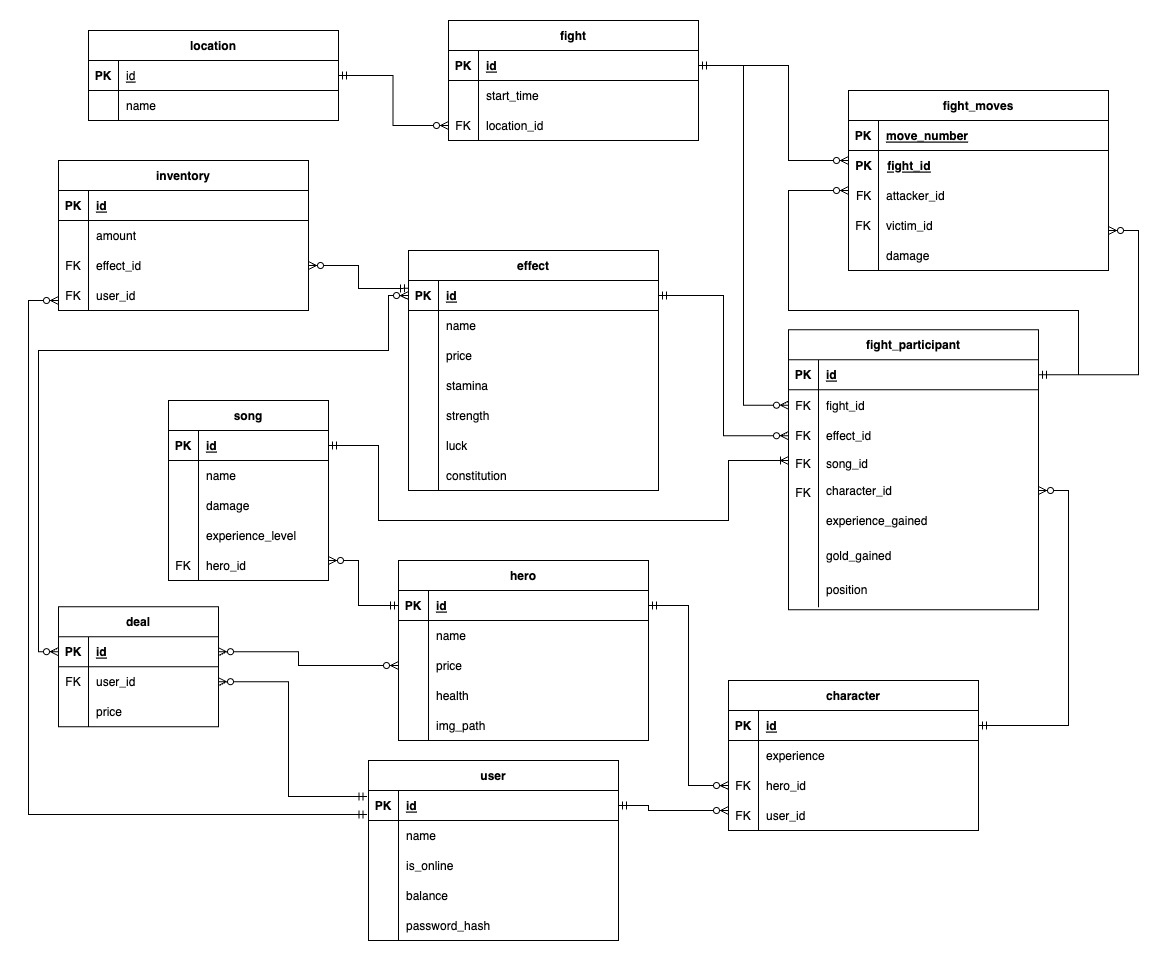
\includegraphics[scale=0.46]{images/ER.jpg}
		\caption{ER-диаграмма предметной области}
	\end{center}
\end{figure}

\subsection*{На основе ER-модели построить даталогическую модель}

\addcontentsline{toc}{subsection}{На основе ER-модели построить даталогическую модель}

\begin{figure}[H]
	\begin{center}
		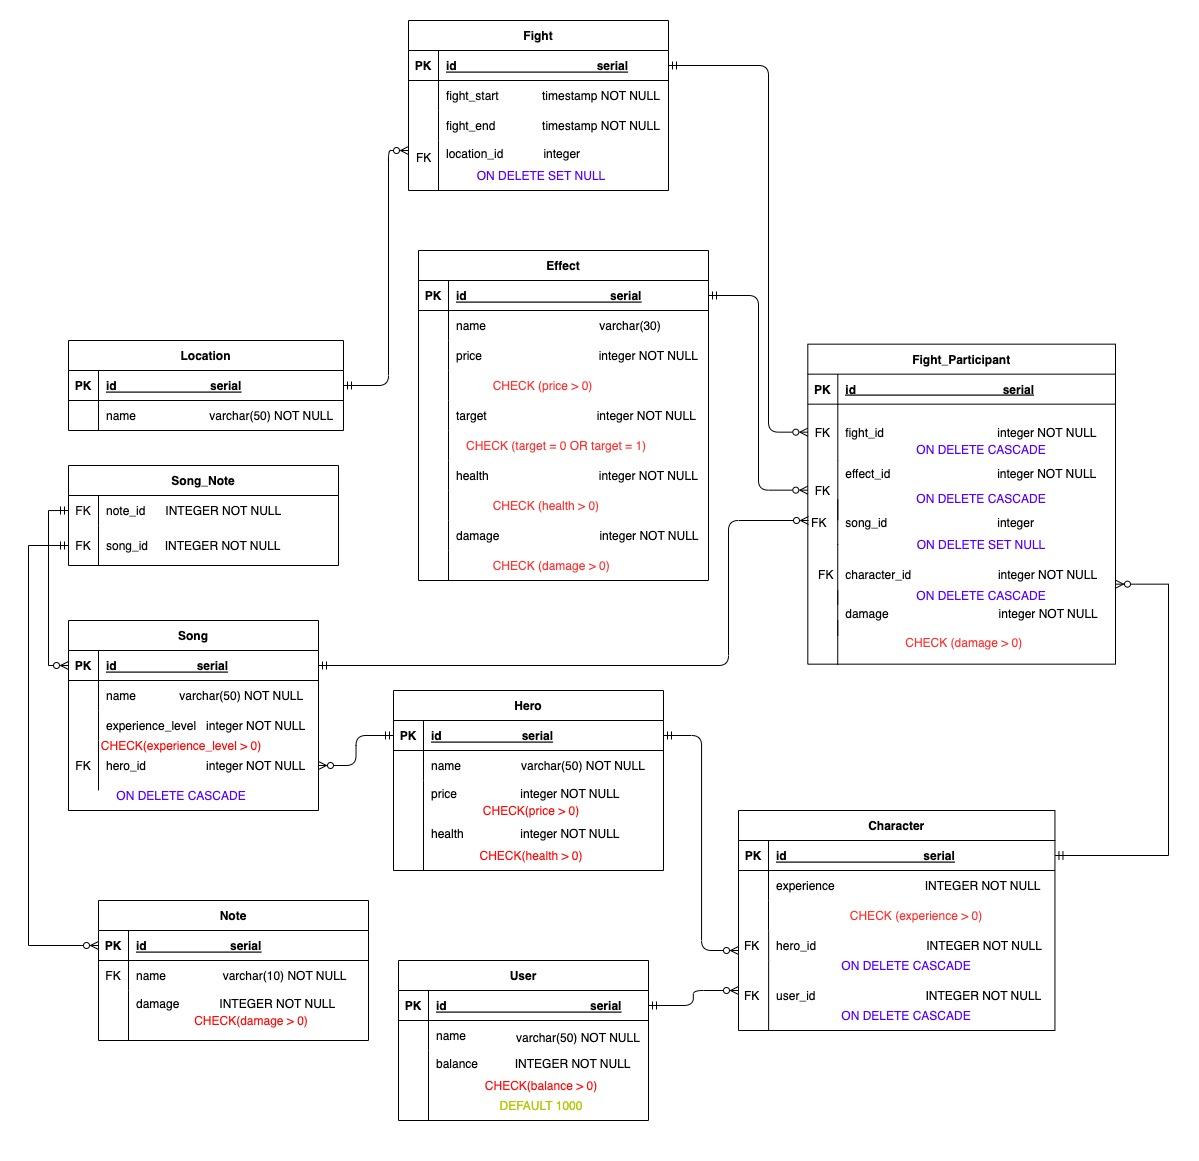
\includegraphics[scale=0.44]{images/Datalogical.jpg}
		\caption{Даталогическая модель}
		\label{pic:pic_name} % название для ссылок внутри кода
	\end{center}
\end{figure}

\newpage

\section*{Этап 3}

\faGithub\href{https://github.com/Vakzu/musical-wars-backend/tree/main/src/main/resources/sql_scripts}{\textbf{Ссылка на код}}

\subsection*{Добавить в базу данных триггеры для обеспечения комплексных ограничений
целостности}

\addcontentsline{toc}{subsection}{Добавить в базу данных триггеры для обеспечения комплексных ограничений
целостности}

\begin{enumerate}
    \item pay\_for\_hero\_log 
    - Тригер для фиксации транзакции игрока за героя(снимает деньги с баланса и добавляет запись в таблицу с транзакциями)

    \item pay\_for\_effect\_log
    - Тригер для фиксации транзакции игрока за эффект(снимает деньги с баланса и добавляет запись в таблицу с транзакциями)
\end{enumerate}

% =====

\subsection*{Реализовать функции и процедуры на основе описания бизнес-процессов}

\addcontentsline{toc}{subsection}{Реализовать функции и процедуры на основе описания бизнес-процессов}

\begin{enumerate}
    \item get\_effect\_shop\_info(user\_id) 
    - Возвращает все эффекты + количество уже купленных игроком

    \item buy\_effect(user\_id, effect\_id)
    - Функция покупки эффекта(eсли у пользователя хватает денег на эффект, то покупаем эффект вычитая стоимость из баланса и занося в inventory)

    \item buy\_hero(user\_id, hero\_id)
    - Функция покупки персонажа(если у игрока хватает денег, то вычитаем стоимость персонажа из баланса и добавляем героя связывая с игроком)

    \item get\_base\_character\_info(character\_id, song\_id)
    - Возвращает основную информацию по герою(id, id игрока, id\_в\_драке, здоровье, урон, выносливость, удача)

    \item get\_shop\_info\_for\_user(user\_id)
    - Возвращает список доступных для покупки героев с их характеристиками(id, имя, цена, здоровье, аватарка, id\_игрока) и статусом куплен или нет.

    \item get\_characters\_info\_with\_songs(character\_id[], song\_id[])
    - Возвращает список информаций по участникам драки основываясь участниках и их песнях

    \item get\_upgrade\_character\_info(participant\_info, effect\_id)
    - Возвращает информацию по персонажу с учетом примененного эффекта.

    \item get\_available\_effects\_for\_user(user\_id)
    - Выводит список доступных(купленных) эффектов для выбора для игрока

    \item get\_available\_songs\_for\_character(character\_id)
    - Выводит список доступных песен для героя

    \item begin\_fight(character\_id[], effect\_id[], song\_id[], location\_id)
    - Функция для начала сражения(прогоняет весь матч и возвращает таблицу ходов)

\end{enumerate}

\newpage

\subsection*{Анализ наиболее часто используемых запросов}

\addcontentsline{toc}{subsection}{Анализ наиболее часто используемых запросов}

Наиболее частыми запросами являются запросы к сущностям 
\begin{itemize}
    \item \textbf{user}
    \begin{itemize}
        \item По \textbf{is\_online}
        \item По \textbf{name}
    \end{itemize}
    Потенциально полезным будет использовать hash index для атрибута \textbf{name}, так как происходит выборка по эквивалентности.

    Добавление индекса для атрибута \textbf{is\_online} бесполезно и не несёт смысла так как значений всего два.
    
    \item \textbf{character}
    \begin{itemize}
        \item По \textbf{user\_id}
        \item По \textbf{id}
    \end{itemize}

    Потенциально полезным будет использовать hash index для атрибута \textbf{user\_id} и \textbf{id}, так как происходит выборка по эквивалентности.

    \item \textbf{hero}
    \begin{itemize}
        \item По \textbf{id}
    \end{itemize}

    Потнциально полезным будет использовать hash index для атрибута \textbf{id}, так как происходит выборка по эквивалентности.

    \item \textbf{effect}
    \begin{itemize}
        \item По \textbf{id}
    \end{itemize}

    Потнциально полезным будет использовать hash index для атрибута \textbf{id}, так как происходит выборка по эквивалентности.

    \item \textbf{inventory}
    \begin{itemize}
        \item По \textbf{user\_id}
        \item По \textbf{effect\_id}
    \end{itemize}

    Потнциально полезным будет использовать hash index для атрибута \textbf{user\_id} и \textbf{effect\_id}, так как происходит выборка по эквивалентности.
\end{itemize}

\subsection*{Доказательство того, что индексы действительно полезны}

\addcontentsline{toc}{subsection}{Доказательство того, что индексы действительно полезны}

\begin{itemize}
    \item Hash index на user(name)
    
    \item Hash index на character(user\_id)
    
    \item Hash index на character(id)

    \item Hash index на hero(id)

    \item Hash index на effect(id)

    \item Hash index на inventory(user\_id)

    \item Hash index на inventory(effect\_id)
\end{itemize}
